\documentclass[]{article}
\usepackage{lmodern}
\usepackage{amssymb,amsmath}
\usepackage{ifxetex,ifluatex}
\usepackage{fixltx2e} % provides \textsubscript
\ifnum 0\ifxetex 1\fi\ifluatex 1\fi=0 % if pdftex
  \usepackage[T1]{fontenc}
  \usepackage[utf8]{inputenc}
\else % if luatex or xelatex
  \ifxetex
    \usepackage{mathspec}
  \else
    \usepackage{fontspec}
  \fi
  \defaultfontfeatures{Ligatures=TeX,Scale=MatchLowercase}
\fi
% use upquote if available, for straight quotes in verbatim environments
\IfFileExists{upquote.sty}{\usepackage{upquote}}{}
% use microtype if available
\IfFileExists{microtype.sty}{%
\usepackage{microtype}
\UseMicrotypeSet[protrusion]{basicmath} % disable protrusion for tt fonts
}{}
\usepackage[margin=1in]{geometry}
\usepackage{hyperref}
\hypersetup{unicode=true,
            pdftitle={Final\_Wrangling\_Doc},
            pdfauthor={BGRR},
            pdfborder={0 0 0},
            breaklinks=true}
\urlstyle{same}  % don't use monospace font for urls
\usepackage{color}
\usepackage{fancyvrb}
\newcommand{\VerbBar}{|}
\newcommand{\VERB}{\Verb[commandchars=\\\{\}]}
\DefineVerbatimEnvironment{Highlighting}{Verbatim}{commandchars=\\\{\}}
% Add ',fontsize=\small' for more characters per line
\usepackage{framed}
\definecolor{shadecolor}{RGB}{248,248,248}
\newenvironment{Shaded}{\begin{snugshade}}{\end{snugshade}}
\newcommand{\AlertTok}[1]{\textcolor[rgb]{0.94,0.16,0.16}{#1}}
\newcommand{\AnnotationTok}[1]{\textcolor[rgb]{0.56,0.35,0.01}{\textbf{\textit{#1}}}}
\newcommand{\AttributeTok}[1]{\textcolor[rgb]{0.77,0.63,0.00}{#1}}
\newcommand{\BaseNTok}[1]{\textcolor[rgb]{0.00,0.00,0.81}{#1}}
\newcommand{\BuiltInTok}[1]{#1}
\newcommand{\CharTok}[1]{\textcolor[rgb]{0.31,0.60,0.02}{#1}}
\newcommand{\CommentTok}[1]{\textcolor[rgb]{0.56,0.35,0.01}{\textit{#1}}}
\newcommand{\CommentVarTok}[1]{\textcolor[rgb]{0.56,0.35,0.01}{\textbf{\textit{#1}}}}
\newcommand{\ConstantTok}[1]{\textcolor[rgb]{0.00,0.00,0.00}{#1}}
\newcommand{\ControlFlowTok}[1]{\textcolor[rgb]{0.13,0.29,0.53}{\textbf{#1}}}
\newcommand{\DataTypeTok}[1]{\textcolor[rgb]{0.13,0.29,0.53}{#1}}
\newcommand{\DecValTok}[1]{\textcolor[rgb]{0.00,0.00,0.81}{#1}}
\newcommand{\DocumentationTok}[1]{\textcolor[rgb]{0.56,0.35,0.01}{\textbf{\textit{#1}}}}
\newcommand{\ErrorTok}[1]{\textcolor[rgb]{0.64,0.00,0.00}{\textbf{#1}}}
\newcommand{\ExtensionTok}[1]{#1}
\newcommand{\FloatTok}[1]{\textcolor[rgb]{0.00,0.00,0.81}{#1}}
\newcommand{\FunctionTok}[1]{\textcolor[rgb]{0.00,0.00,0.00}{#1}}
\newcommand{\ImportTok}[1]{#1}
\newcommand{\InformationTok}[1]{\textcolor[rgb]{0.56,0.35,0.01}{\textbf{\textit{#1}}}}
\newcommand{\KeywordTok}[1]{\textcolor[rgb]{0.13,0.29,0.53}{\textbf{#1}}}
\newcommand{\NormalTok}[1]{#1}
\newcommand{\OperatorTok}[1]{\textcolor[rgb]{0.81,0.36,0.00}{\textbf{#1}}}
\newcommand{\OtherTok}[1]{\textcolor[rgb]{0.56,0.35,0.01}{#1}}
\newcommand{\PreprocessorTok}[1]{\textcolor[rgb]{0.56,0.35,0.01}{\textit{#1}}}
\newcommand{\RegionMarkerTok}[1]{#1}
\newcommand{\SpecialCharTok}[1]{\textcolor[rgb]{0.00,0.00,0.00}{#1}}
\newcommand{\SpecialStringTok}[1]{\textcolor[rgb]{0.31,0.60,0.02}{#1}}
\newcommand{\StringTok}[1]{\textcolor[rgb]{0.31,0.60,0.02}{#1}}
\newcommand{\VariableTok}[1]{\textcolor[rgb]{0.00,0.00,0.00}{#1}}
\newcommand{\VerbatimStringTok}[1]{\textcolor[rgb]{0.31,0.60,0.02}{#1}}
\newcommand{\WarningTok}[1]{\textcolor[rgb]{0.56,0.35,0.01}{\textbf{\textit{#1}}}}
\usepackage{graphicx,grffile}
\makeatletter
\def\maxwidth{\ifdim\Gin@nat@width>\linewidth\linewidth\else\Gin@nat@width\fi}
\def\maxheight{\ifdim\Gin@nat@height>\textheight\textheight\else\Gin@nat@height\fi}
\makeatother
% Scale images if necessary, so that they will not overflow the page
% margins by default, and it is still possible to overwrite the defaults
% using explicit options in \includegraphics[width, height, ...]{}
\setkeys{Gin}{width=\maxwidth,height=\maxheight,keepaspectratio}
\IfFileExists{parskip.sty}{%
\usepackage{parskip}
}{% else
\setlength{\parindent}{0pt}
\setlength{\parskip}{6pt plus 2pt minus 1pt}
}
\setlength{\emergencystretch}{3em}  % prevent overfull lines
\providecommand{\tightlist}{%
  \setlength{\itemsep}{0pt}\setlength{\parskip}{0pt}}
\setcounter{secnumdepth}{0}
% Redefines (sub)paragraphs to behave more like sections
\ifx\paragraph\undefined\else
\let\oldparagraph\paragraph
\renewcommand{\paragraph}[1]{\oldparagraph{#1}\mbox{}}
\fi
\ifx\subparagraph\undefined\else
\let\oldsubparagraph\subparagraph
\renewcommand{\subparagraph}[1]{\oldsubparagraph{#1}\mbox{}}
\fi

%%% Use protect on footnotes to avoid problems with footnotes in titles
\let\rmarkdownfootnote\footnote%
\def\footnote{\protect\rmarkdownfootnote}

%%% Change title format to be more compact
\usepackage{titling}

% Create subtitle command for use in maketitle
\providecommand{\subtitle}[1]{
  \posttitle{
    \begin{center}\large#1\end{center}
    }
}

\setlength{\droptitle}{-2em}

  \title{Final\_Wrangling\_Doc}
    \pretitle{\vspace{\droptitle}\centering\huge}
  \posttitle{\par}
    \author{BGRR}
    \preauthor{\centering\large\emph}
  \postauthor{\par}
      \predate{\centering\large\emph}
  \postdate{\par}
    \date{11/11/2019}


\begin{document}
\maketitle

\begin{Shaded}
\begin{Highlighting}[]
\KeywordTok{getwd}\NormalTok{()}
\end{Highlighting}
\end{Shaded}

\begin{verbatim}
## [1] "C:/Users/Felipe/OneDrive - Duke University/1. DUKE/Ramos 3 Semestre/722 Hydro Data/HDA_Project_FRA"
\end{verbatim}

\begin{Shaded}
\begin{Highlighting}[]
\CommentTok{#load packages}
\KeywordTok{library}\NormalTok{(tidyverse)}
\end{Highlighting}
\end{Shaded}

\begin{verbatim}
## -- Attaching packages ------------------------------------------ tidyverse 1.2.1 --
\end{verbatim}

\begin{verbatim}
## v ggplot2 3.2.1     v purrr   0.3.2
## v tibble  2.1.3     v dplyr   0.8.3
## v tidyr   0.8.3     v stringr 1.4.0
## v readr   1.3.1     v forcats 0.4.0
\end{verbatim}

\begin{verbatim}
## -- Conflicts --------------------------------------------- tidyverse_conflicts() --
## x dplyr::filter() masks stats::filter()
## x dplyr::lag()    masks stats::lag()
\end{verbatim}

\begin{Shaded}
\begin{Highlighting}[]
\KeywordTok{library}\NormalTok{(lubridate)}
\end{Highlighting}
\end{Shaded}

\begin{verbatim}
## 
## Attaching package: 'lubridate'
\end{verbatim}

\begin{verbatim}
## The following object is masked from 'package:base':
## 
##     date
\end{verbatim}

\begin{Shaded}
\begin{Highlighting}[]
\KeywordTok{library}\NormalTok{(LAGOSNE)}
\KeywordTok{library}\NormalTok{(sf)}
\end{Highlighting}
\end{Shaded}

\begin{verbatim}
## Linking to GEOS 3.6.1, GDAL 2.2.3, PROJ 4.9.3
\end{verbatim}

\begin{Shaded}
\begin{Highlighting}[]
\KeywordTok{library}\NormalTok{(maps)}
\end{Highlighting}
\end{Shaded}

\begin{verbatim}
## 
## Attaching package: 'maps'
\end{verbatim}

\begin{verbatim}
## The following object is masked from 'package:purrr':
## 
##     map
\end{verbatim}

\begin{Shaded}
\begin{Highlighting}[]
\KeywordTok{library}\NormalTok{(mapview)}

\CommentTok{#load LAGOS data}
\NormalTok{LAGOSdata <-}\StringTok{ }\KeywordTok{lagosne_load}\NormalTok{()}
\end{Highlighting}
\end{Shaded}

\begin{verbatim}
## Warning in `_f`(version = version, fpath = fpath): LAGOSNE version
## unspecified, loading version: 1.087.3
\end{verbatim}

\begin{Shaded}
\begin{Highlighting}[]
\CommentTok{# creating specific lagos files}
\NormalTok{LAGOSstate <-}\StringTok{ }\NormalTok{LAGOSdata}\OperatorTok{$}\NormalTok{state}
\NormalTok{LAGOSlocus <-}\StringTok{ }\NormalTok{LAGOSdata}\OperatorTok{$}\NormalTok{locus}
\NormalTok{LAGOSnutrient <-}\StringTok{ }\NormalTok{LAGOSdata}\OperatorTok{$}\NormalTok{epi_nutr}
\NormalTok{LAGOSiwslulc <-}\StringTok{ }\NormalTok{LAGOSdata}\OperatorTok{$}\NormalTok{iws.lulc}
\NormalTok{LAGOSiws <-}\StringTok{ }\NormalTok{LAGOSdata}\OperatorTok{$}\NormalTok{iws}

\KeywordTok{theme_set}\NormalTok{(}\KeywordTok{theme_classic}\NormalTok{())}
\end{Highlighting}
\end{Shaded}

\begin{Shaded}
\begin{Highlighting}[]
\CommentTok{#checking each state for nutrient data}

\CommentTok{#State 14: Minnesota}
\NormalTok{LAGOSlocus.MN <-}\StringTok{ }\NormalTok{LAGOSlocus }\OperatorTok\StringTok{ }\KeywordTok{filter}\NormalTok{ (state_zoneid }\OperatorTok{==}\StringTok{ "State_14"}\NormalTok{)}
\NormalTok{LAGOSnutrient.MN <-}\StringTok{ }\NormalTok{LAGOSlocus.MN }\OperatorTok
\StringTok{  }\KeywordTok{left_join}\NormalTok{(LAGOSnutrient, }\DataTypeTok{by =} \StringTok{"lagoslakeid"}\NormalTok{) }
\end{Highlighting}
\end{Shaded}

\begin{Shaded}
\begin{Highlighting}[]
\CommentTok{#getting the area of the iws}
\NormalTok{LAGOSiws.area <-}\StringTok{ }\KeywordTok{select}\NormalTok{(LAGOSiws, }\StringTok{"lagoslakeid"}\NormalTok{, }\StringTok{"iws_ha"}\NormalTok{)}


\CommentTok{#joining MN locus with iwslulc and adding the area of IWS}
\NormalTok{LAGOSiws.MN <-}\StringTok{ }\NormalTok{LAGOSlocus.MN }\OperatorTok\StringTok{ }
\StringTok{  }\KeywordTok{left_join}\NormalTok{(LAGOSiwslulc, }\DataTypeTok{by =} \StringTok{"lagoslakeid"}\NormalTok{) }\OperatorTok
\StringTok{  }\KeywordTok{left_join}\NormalTok{(LAGOSiws.area, }\DataTypeTok{by =} \StringTok{"lagoslakeid"}\NormalTok{)}

\CommentTok{##selecting 2011 lulc}
\NormalTok{LAGOSiws2011.MN <-}\StringTok{ }\NormalTok{LAGOSiws.MN }\OperatorTok\StringTok{ }
\StringTok{  }\KeywordTok{select}\NormalTok{(lagoslakeid,state_zoneid, lake_area_ha, iws_ha,}
\NormalTok{         iws_nlcd2011_pct_}\DecValTok{11}\NormalTok{, iws_nlcd2011_pct_}\DecValTok{21}\NormalTok{, iws_nlcd2011_pct_}\DecValTok{22}\NormalTok{,}
\NormalTok{         iws_nlcd2011_pct_}\DecValTok{23}\NormalTok{, iws_nlcd2011_pct_}\DecValTok{24}\NormalTok{, iws_nlcd2011_pct_}\DecValTok{31}\NormalTok{,}
\NormalTok{         iws_nlcd2011_pct_}\DecValTok{41}\NormalTok{, iws_nlcd2011_pct_}\DecValTok{42}\NormalTok{, iws_nlcd2011_pct_}\DecValTok{43}\NormalTok{,}
\NormalTok{         iws_nlcd2011_pct_}\DecValTok{52}\NormalTok{, iws_nlcd2011_pct_}\DecValTok{71}\NormalTok{, iws_nlcd2011_pct_}\DecValTok{81}\NormalTok{,}
\NormalTok{         iws_nlcd2011_pct_}\DecValTok{82}\NormalTok{, iws_nlcd2011_pct_}\DecValTok{90}\NormalTok{, iws_nlcd2011_pct_}\DecValTok{95}\NormalTok{)}
\end{Highlighting}
\end{Shaded}

\begin{Shaded}
\begin{Highlighting}[]
\CommentTok{#filtering state nutrient data #FRA. We can expand this range}
\NormalTok{LAGOSnutrient.MN.skinny <-}\StringTok{ }\NormalTok{LAGOSnutrient.MN }\OperatorTok
\StringTok{  }\KeywordTok{filter}\NormalTok{(sampledate }\OperatorTok{>}\StringTok{ "2008-12-31"} \OperatorTok{&}\StringTok{ }\NormalTok{sampledate }\OperatorTok{<}\StringTok{ "2015-01-01"}\NormalTok{)}

\CommentTok{# sapply(LAGOSnutrient.MN.skinny, summary)}
\end{Highlighting}
\end{Shaded}

\begin{Shaded}
\begin{Highlighting}[]
\CommentTok{##Joining iws.lulc and nutrient}
\NormalTok{LAGOSiws.nutrient.}\FloatTok{2011.}\NormalTok{MN <-}\StringTok{  }\KeywordTok{left_join}\NormalTok{(LAGOSnutrient.MN.skinny,}
\NormalTok{                                        LAGOSiws2011.MN, }\DataTypeTok{by =}
                                          \KeywordTok{c}\NormalTok{(}\StringTok{"lagoslakeid"}\NormalTok{, }\StringTok{"lake_area_ha"}\NormalTok{)) }

\NormalTok{LAGOSiws.nutrient.}\FloatTok{2011.}\NormalTok{MN <-}\StringTok{ }\NormalTok{LAGOSiws.nutrient.}\FloatTok{2011.}\NormalTok{MN }\OperatorTok
\StringTok{  }\KeywordTok{select}\NormalTok{(lagoslakeid, nhd_lat, nhd_long, lake_area_ha, lake_perim_meters,}
\NormalTok{         iws_zoneid, iws_ha, state_zoneid.x, elevation_m, sampledate, chla,secchi, }
\NormalTok{         iws_nlcd2011_pct_}\DecValTok{11}\NormalTok{, iws_nlcd2011_pct_}\DecValTok{21}\NormalTok{, iws_nlcd2011_pct_}\DecValTok{22}\NormalTok{, }
\NormalTok{         iws_nlcd2011_pct_}\DecValTok{23}\NormalTok{, iws_nlcd2011_pct_}\DecValTok{24}\NormalTok{, iws_nlcd2011_pct_}\DecValTok{31}\NormalTok{, }
\NormalTok{         iws_nlcd2011_pct_}\DecValTok{41}\NormalTok{, iws_nlcd2011_pct_}\DecValTok{42}\NormalTok{, iws_nlcd2011_pct_}\DecValTok{43}\NormalTok{, }
\NormalTok{         iws_nlcd2011_pct_}\DecValTok{52}\NormalTok{, iws_nlcd2011_pct_}\DecValTok{71}\NormalTok{, iws_nlcd2011_pct_}\DecValTok{81}\NormalTok{, }
\NormalTok{         iws_nlcd2011_pct_}\DecValTok{82}\NormalTok{, iws_nlcd2011_pct_}\DecValTok{90}\NormalTok{, iws_nlcd2011_pct_}\DecValTok{95}\NormalTok{)}

\CommentTok{# sapply(LAGOSiws.nutrient.2011.MN, summary)}
\end{Highlighting}
\end{Shaded}

\begin{Shaded}
\begin{Highlighting}[]
\CommentTok{# Looking at the data}

\KeywordTok{ggplot}\NormalTok{(LAGOSiws.nutrient.}\FloatTok{2011.}\NormalTok{MN, }\KeywordTok{aes}\NormalTok{(}\DataTypeTok{x =}\NormalTok{ sampledate, }\DataTypeTok{y =}\NormalTok{ secchi, }\DataTypeTok{color =}\NormalTok{ lagoslakeid)) }\OperatorTok{+}
\StringTok{  }\KeywordTok{scale_color_viridis_c}\NormalTok{(}\DataTypeTok{option =} \StringTok{"plasma"}\NormalTok{) }\OperatorTok{+}
\StringTok{  }\KeywordTok{geom_line}\NormalTok{() }
\end{Highlighting}
\end{Shaded}

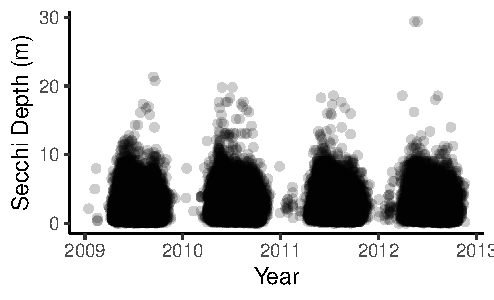
\includegraphics{Final_Wrangling_Doc_files/figure-latex/Visualize_data-1.pdf}

\begin{Shaded}
\begin{Highlighting}[]
\KeywordTok{ggplot}\NormalTok{(LAGOSiws.nutrient.}\FloatTok{2011.}\NormalTok{MN, }\KeywordTok{aes}\NormalTok{(}\DataTypeTok{x =}\NormalTok{ sampledate, }\DataTypeTok{y =}\NormalTok{ chla, }\DataTypeTok{color =}\NormalTok{ lagoslakeid)) }\OperatorTok{+}
\StringTok{  }\KeywordTok{scale_color_viridis_c}\NormalTok{(}\DataTypeTok{option =} \StringTok{"plasma"}\NormalTok{) }\OperatorTok{+}
\StringTok{  }\KeywordTok{geom_line}\NormalTok{() }
\end{Highlighting}
\end{Shaded}

\begin{verbatim}
## Warning: Removed 10 rows containing missing values (geom_path).
\end{verbatim}

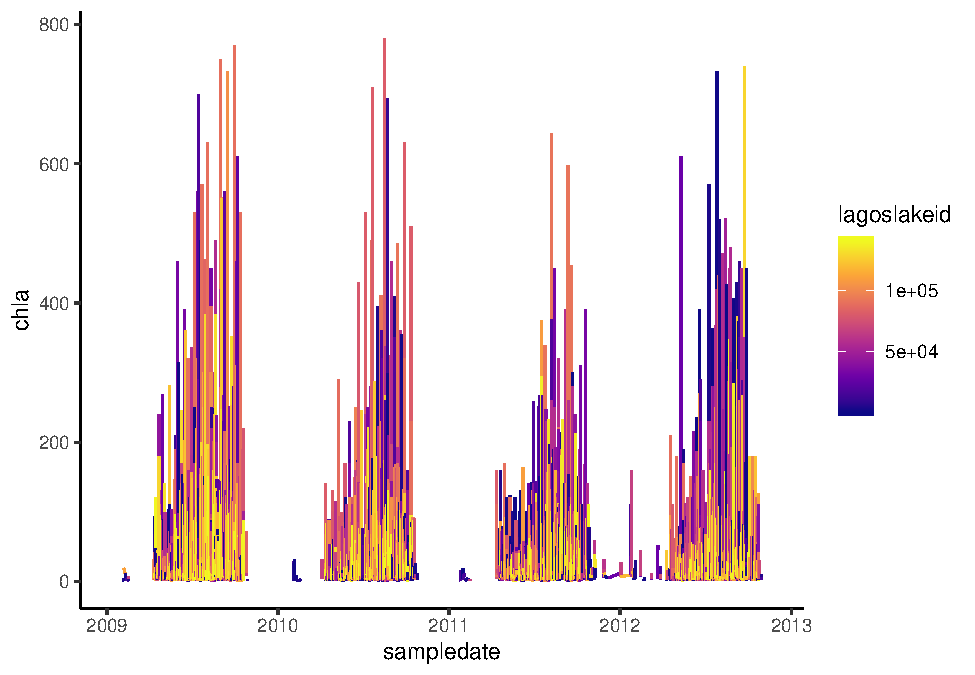
\includegraphics{Final_Wrangling_Doc_files/figure-latex/Visualize_data-2.pdf}

\begin{Shaded}
\begin{Highlighting}[]
\NormalTok{LAGOS.MN.processed <-}\StringTok{ }\NormalTok{LAGOSiws.nutrient.}\FloatTok{2011.}\NormalTok{MN }\OperatorTok
\StringTok{  }\KeywordTok{mutate}\NormalTok{(}\DataTypeTok{Water.pct =}\NormalTok{ iws_nlcd2011_pct_}\DecValTok{11}\NormalTok{,}
         \DataTypeTok{Urban.pct =}\NormalTok{ iws_nlcd2011_pct_}\DecValTok{21} \OperatorTok{+}\StringTok{ }\NormalTok{iws_nlcd2011_pct_}\DecValTok{22} \OperatorTok{+}
\StringTok{           }\NormalTok{iws_nlcd2011_pct_}\DecValTok{23} \OperatorTok{+}\StringTok{ }\NormalTok{iws_nlcd2011_pct_}\DecValTok{24}\NormalTok{,}
         \DataTypeTok{Undeveloped.pct =}\NormalTok{ iws_nlcd2011_pct_}\DecValTok{31} \OperatorTok{+}\StringTok{ }\NormalTok{iws_nlcd2011_pct_}\DecValTok{41} \OperatorTok{+}
\StringTok{           }\NormalTok{iws_nlcd2011_pct_}\DecValTok{42} \OperatorTok{+}\StringTok{ }\NormalTok{iws_nlcd2011_pct_}\DecValTok{43} \OperatorTok{+}\StringTok{ }
\StringTok{           }\NormalTok{iws_nlcd2011_pct_}\DecValTok{52} \OperatorTok{+}\StringTok{ }\NormalTok{iws_nlcd2011_pct_}\DecValTok{90} \OperatorTok{+}\StringTok{ }\NormalTok{iws_nlcd2011_pct_}\DecValTok{95}\NormalTok{,}
         \DataTypeTok{Ag.pct =}\NormalTok{  iws_nlcd2011_pct_}\DecValTok{81} \OperatorTok{+}\StringTok{ }\NormalTok{iws_nlcd2011_pct_}\DecValTok{82} \OperatorTok{+}\StringTok{ }\NormalTok{iws_nlcd2011_pct_}\DecValTok{71}\NormalTok{) }\OperatorTok
\StringTok{  }\KeywordTok{select}\NormalTok{(}\OperatorTok{-}\KeywordTok{c}\NormalTok{(iws_nlcd2011_pct_}\DecValTok{11}\NormalTok{, iws_nlcd2011_pct_}\DecValTok{21}\NormalTok{, iws_nlcd2011_pct_}\DecValTok{22}\NormalTok{, }
\NormalTok{            iws_nlcd2011_pct_}\DecValTok{23}\NormalTok{, iws_nlcd2011_pct_}\DecValTok{24}\NormalTok{, iws_nlcd2011_pct_}\DecValTok{31}\NormalTok{, }
\NormalTok{            iws_nlcd2011_pct_}\DecValTok{41}\NormalTok{, iws_nlcd2011_pct_}\DecValTok{42}\NormalTok{, iws_nlcd2011_pct_}\DecValTok{43}\NormalTok{, }
\NormalTok{            iws_nlcd2011_pct_}\DecValTok{52}\NormalTok{, iws_nlcd2011_pct_}\DecValTok{71}\NormalTok{, iws_nlcd2011_pct_}\DecValTok{81}\NormalTok{, }
\NormalTok{            iws_nlcd2011_pct_}\DecValTok{82}\NormalTok{, iws_nlcd2011_pct_}\DecValTok{90}\NormalTok{, iws_nlcd2011_pct_}\DecValTok{95}\NormalTok{)) }\OperatorTok
\StringTok{  }\KeywordTok{na.omit}\NormalTok{() }\OperatorTok
\StringTok{  }\KeywordTok{mutate}\NormalTok{(}\DataTypeTok{LakeIWS.Ratio =}\NormalTok{ lake_area_ha}\OperatorTok{/}\NormalTok{iws_ha) }\OperatorTok
\StringTok{  }\KeywordTok{mutate}\NormalTok{(}\DataTypeTok{DOY =} \KeywordTok{yday}\NormalTok{(sampledate))}
  
\CommentTok{# sapply(LAGOS.MN.processed, summary)}
\end{Highlighting}
\end{Shaded}

\begin{Shaded}
\begin{Highlighting}[]
\CommentTok{#We are creating growing seasons; early, prime, late. They will be based off of water temperature and day of year. We choose May 15 and October 1 because these are arbitrary but approximate bookends to the prime growing season.}

\NormalTok{LAGOS.MN.processed}\OperatorTok{$}\NormalTok{EarlyTrue <-}\StringTok{ }\NormalTok{LAGOS.MN.processed}\OperatorTok{$}\NormalTok{DOY }\OperatorTok{<}\StringTok{ }\DecValTok{136} \CommentTok{#Before May 15}
\NormalTok{LAGOS.MN.processed}\OperatorTok{$}\NormalTok{PrimeTrue <-}\StringTok{ }\NormalTok{LAGOS.MN.processed}\OperatorTok{$}\NormalTok{DOY }\OperatorTok{>=}\DecValTok{136} \OperatorTok{&}\StringTok{ }\NormalTok{LAGOS.MN.processed}\OperatorTok{$}\NormalTok{DOY }\OperatorTok{<=}\StringTok{ }\DecValTok{273} \CommentTok{#May 15 to September 30}
\NormalTok{LAGOS.MN.processed}\OperatorTok{$}\NormalTok{LateTrue <-}\StringTok{ }\NormalTok{LAGOS.MN.processed}\OperatorTok{$}\NormalTok{DOY }\OperatorTok{>}\StringTok{ }\DecValTok{273}  \CommentTok{#October 1 and later}

\NormalTok{LAGOS.MN.processed}\OperatorTok{$}\NormalTok{EarlyTrue <-}\StringTok{ }\KeywordTok{ifelse}\NormalTok{(LAGOS.MN.processed}\OperatorTok{$}\NormalTok{EarlyTrue }\OperatorTok{==}\StringTok{ }\OtherTok{TRUE}\NormalTok{, }\StringTok{"Early"}\NormalTok{, }\StringTok{"No"}\NormalTok{)}
\NormalTok{LAGOS.MN.processed}\OperatorTok{$}\NormalTok{PrimeTrue <-}\StringTok{ }\KeywordTok{ifelse}\NormalTok{(LAGOS.MN.processed}\OperatorTok{$}\NormalTok{PrimeTrue }\OperatorTok{==}\StringTok{ }\OtherTok{TRUE}\NormalTok{, }\StringTok{"Prime"}\NormalTok{, }\StringTok{"No"}\NormalTok{)}
\NormalTok{LAGOS.MN.processed}\OperatorTok{$}\NormalTok{LateTrue <-}\StringTok{ }\KeywordTok{ifelse}\NormalTok{(LAGOS.MN.processed}\OperatorTok{$}\NormalTok{LateTrue }\OperatorTok{==}\StringTok{ }\OtherTok{TRUE}\NormalTok{, }\StringTok{"Late"}\NormalTok{, }\StringTok{"No"}\NormalTok{)}

\NormalTok{LAGOS.MN.processed}\OperatorTok{$}\NormalTok{Season <-}\StringTok{ }\NormalTok{LAGOS.MN.processed}\OperatorTok{$}\NormalTok{EarlyTrue }\OperatorTok{==}\StringTok{ "Early"}
  
\NormalTok{LAGOS.MN.processed}\OperatorTok{$}\NormalTok{Season[LAGOS.MN.processed}\OperatorTok{$}\NormalTok{EarlyTrue }\OperatorTok{==}\StringTok{ "Early"}\NormalTok{] <-}\StringTok{ "Early"}
\NormalTok{LAGOS.MN.processed}\OperatorTok{$}\NormalTok{Season[LAGOS.MN.processed}\OperatorTok{$}\NormalTok{PrimeTrue }\OperatorTok{==}\StringTok{ "Prime"}\NormalTok{] <-}\StringTok{ "Prime"}
\NormalTok{LAGOS.MN.processed}\OperatorTok{$}\NormalTok{Season[LAGOS.MN.processed}\OperatorTok{$}\NormalTok{LateTrue }\OperatorTok{==}\StringTok{ "Late"}\NormalTok{] <-}\StringTok{ "Late"}

\NormalTok{LAGOS.MN.processed  <-}\StringTok{ }\NormalTok{LAGOS.MN.processed }\OperatorTok
\StringTok{  }\KeywordTok{select}\NormalTok{(}\OperatorTok{-}\KeywordTok{c}\NormalTok{(EarlyTrue, PrimeTrue, LateTrue))}
\end{Highlighting}
\end{Shaded}

\begin{Shaded}
\begin{Highlighting}[]
\NormalTok{LAGOS.MN.processed.sf <-}\StringTok{ }\KeywordTok{st_as_sf}\NormalTok{(LAGOS.MN.processed, }\DataTypeTok{coords =} \KeywordTok{c}\NormalTok{(}\StringTok{"nhd_long"}\NormalTok{, }\StringTok{"nhd_lat"}\NormalTok{), }\DataTypeTok{crs =} \DecValTok{4326}\NormalTok{)}

\NormalTok{LAGOS.MN.processed.UTM.sf <-}\StringTok{ }\KeywordTok{st_transform}\NormalTok{(LAGOS.MN.processed.sf, }\DataTypeTok{crs=}\DecValTok{26917}\NormalTok{)}

\NormalTok{MN.Ecoregions.sf <-}\StringTok{ }\KeywordTok{st_read}\NormalTok{(}\StringTok{'./Data/Raw/mn_eco_l3.shp'}\NormalTok{)}
\end{Highlighting}
\end{Shaded}

\begin{verbatim}
## Reading layer `mn_eco_l3' from data source `C:\Users\Felipe\OneDrive - Duke University\1. DUKE\Ramos 3 Semestre\722 Hydro Data\HDA_Project_FRA\data\raw\mn_eco_l3.shp' using driver `ESRI Shapefile'
## Simple feature collection with 7 features and 13 fields
## geometry type:  MULTIPOLYGON
## dimension:      XY
## bbox:           xmin: -91854.57 ymin: 2278542 xmax: 489296.4 ymax: 2930681
## epsg (SRID):    NA
## proj4string:    +proj=aea +lat_1=29.5 +lat_2=45.5 +lat_0=23 +lon_0=-96 +x_0=0 +y_0=0 +datum=NAD83 +units=m +no_defs
\end{verbatim}

\begin{Shaded}
\begin{Highlighting}[]
\CommentTok{#Selecting level 3 ecoregions names}
\NormalTok{MN.Ecoregions.sf <-}\StringTok{ }\KeywordTok{select}\NormalTok{(MN.Ecoregions.sf, US_L3NAME)}

\CommentTok{#mapview(MN.Ecoregions.sf)}

\NormalTok{MN.Ecoregions.UTM.sf <-}\StringTok{ }\KeywordTok{st_transform}\NormalTok{(MN.Ecoregions.sf, }\DataTypeTok{crs=}\DecValTok{26917}\NormalTok{)}

\NormalTok{LAGOS.MN.processed.sf <-}\StringTok{ }\KeywordTok{st_join}\NormalTok{(LAGOS.MN.processed.UTM.sf, MN.Ecoregions.UTM.sf)}
\end{Highlighting}
\end{Shaded}

\begin{Shaded}
\begin{Highlighting}[]
\CommentTok{#Creating sf seasons files}
\NormalTok{LAGOS.MN.processed.Early.sf <-}\StringTok{ }\KeywordTok{filter}\NormalTok{(LAGOS.MN.processed.sf, Season }\OperatorTok{==}\StringTok{ "Early"}\NormalTok{)}
\NormalTok{LAGOS.MN.processed.Prime.sf <-}\StringTok{ }\KeywordTok{filter}\NormalTok{(LAGOS.MN.processed.sf, Season }\OperatorTok{==}\StringTok{ "Prime"}\NormalTok{)}
\NormalTok{LAGOS.MN.processed.Late.sf <-}\StringTok{ }\KeywordTok{filter}\NormalTok{(LAGOS.MN.processed.sf, Season }\OperatorTok{==}\StringTok{ "Late"}\NormalTok{)}

\CommentTok{#Creating regular season files (doesn't have ecoregions column)}
\NormalTok{LAGOS.MN.processed.Early <-}\StringTok{ }\KeywordTok{filter}\NormalTok{(LAGOS.MN.processed, Season }\OperatorTok{==}\StringTok{ "Early"}\NormalTok{)}
\NormalTok{LAGOS.MN.processed.Prime <-}\StringTok{ }\KeywordTok{filter}\NormalTok{(LAGOS.MN.processed, Season }\OperatorTok{==}\StringTok{ "Prime"}\NormalTok{)}
\NormalTok{LAGOS.MN.processed.Late <-}\StringTok{ }\KeywordTok{filter}\NormalTok{(LAGOS.MN.processed, Season }\OperatorTok{==}\StringTok{ "Late"}\NormalTok{)}

\CommentTok{# summary(LAGOS.MN.processed.Early.sf$chla)}
\CommentTok{# summary(LAGOS.MN.processed.Prime.sf$chla)}
\CommentTok{# summary(LAGOS.MN.processed.Late.sf$chla)}
\CommentTok{# }
\CommentTok{# summary(LAGOS.MN.processed.Early.sf$secchi)}
\CommentTok{# summary(LAGOS.MN.processed.Prime.sf$secchi)}
\CommentTok{# summary(LAGOS.MN.processed.Late.sf$secchi)}
\end{Highlighting}
\end{Shaded}

\begin{Shaded}
\begin{Highlighting}[]
\KeywordTok{ggplot}\NormalTok{(LAGOS.MN.processed.Late.sf, }\KeywordTok{aes}\NormalTok{(}\DataTypeTok{x =}\NormalTok{ Undeveloped.pct, }\DataTypeTok{y =}\NormalTok{ secchi)) }\OperatorTok{+}
\KeywordTok{geom_point}\NormalTok{() }\OperatorTok{+}
\KeywordTok{geom_smooth}\NormalTok{(}\DataTypeTok{method=}\NormalTok{lm) }\OperatorTok{+}
\KeywordTok{xlab}\NormalTok{(}\KeywordTok{expression}\NormalTok{(}\StringTok{"Undeveloped %"}\NormalTok{)) }\OperatorTok{+}
\KeywordTok{ylab}\NormalTok{(}\KeywordTok{expression}\NormalTok{(}\StringTok{"Secchi Depth (m)"}\NormalTok{)) }\OperatorTok{+}
\KeywordTok{ggtitle}\NormalTok{(}\StringTok{"Undeveloped % vs Secchi Depth Scatterplot, Late Season"}\NormalTok{) }\OperatorTok{+}
\KeywordTok{theme}\NormalTok{(}\DataTypeTok{plot.title =} \KeywordTok{element_text}\NormalTok{(}\DataTypeTok{hjust =} \FloatTok{0.5}\NormalTok{))}
\end{Highlighting}
\end{Shaded}

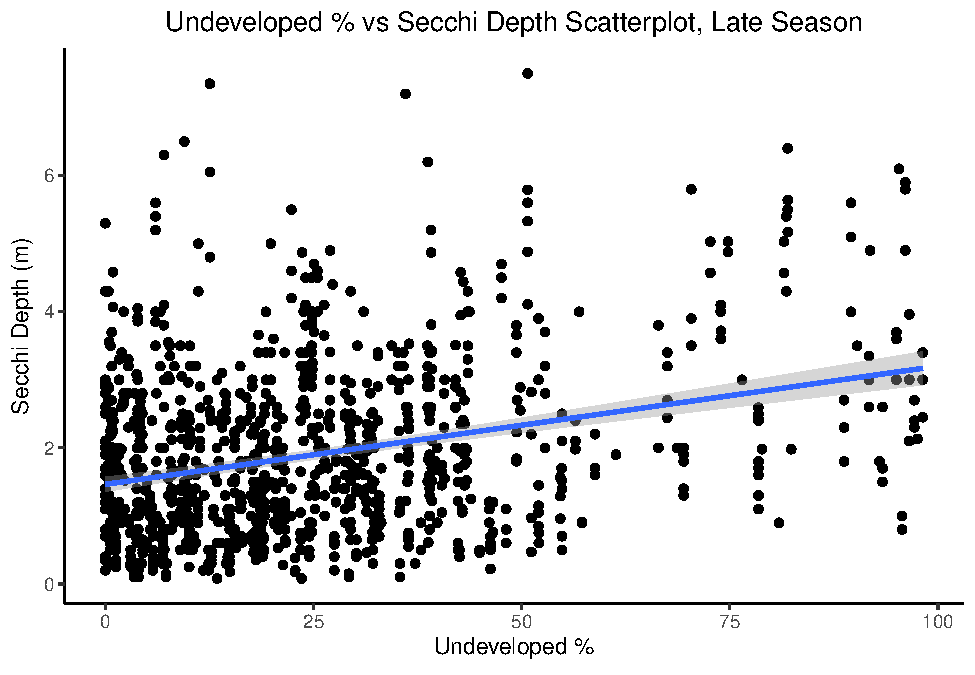
\includegraphics{Final_Wrangling_Doc_files/figure-latex/scatterplots-1.pdf}

\begin{Shaded}
\begin{Highlighting}[]
\KeywordTok{ggplot}\NormalTok{(LAGOS.MN.processed.Late.sf, }\KeywordTok{aes}\NormalTok{(}\DataTypeTok{x =}\NormalTok{ Urban.pct, }\DataTypeTok{y =}\NormalTok{ secchi)) }\OperatorTok{+}
\KeywordTok{geom_point}\NormalTok{() }\OperatorTok{+}
\KeywordTok{geom_smooth}\NormalTok{(}\DataTypeTok{method=}\NormalTok{lm) }\OperatorTok{+}
\KeywordTok{xlab}\NormalTok{(}\KeywordTok{expression}\NormalTok{(}\StringTok{"Urban %"}\NormalTok{)) }\OperatorTok{+}
\KeywordTok{ylab}\NormalTok{(}\KeywordTok{expression}\NormalTok{(}\StringTok{"Secchi Depth (m)"}\NormalTok{)) }\OperatorTok{+}
\KeywordTok{ggtitle}\NormalTok{(}\StringTok{"Urban % vs Secchi Depth Scatterplot, Late Season"}\NormalTok{) }\OperatorTok{+}
\KeywordTok{theme}\NormalTok{(}\DataTypeTok{plot.title =} \KeywordTok{element_text}\NormalTok{(}\DataTypeTok{hjust =} \FloatTok{0.5}\NormalTok{))}
\end{Highlighting}
\end{Shaded}

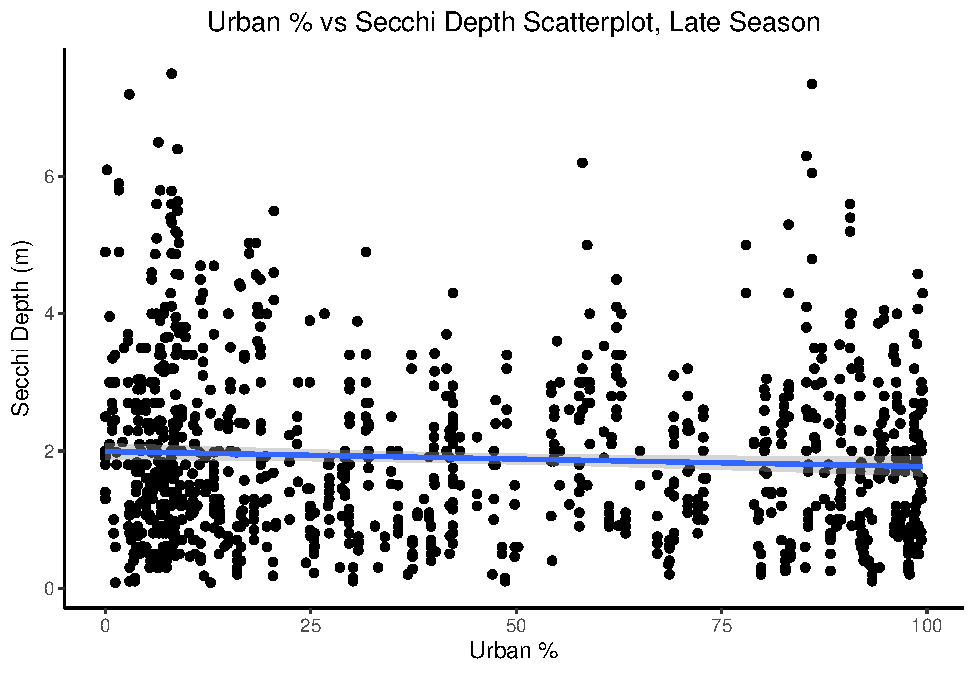
\includegraphics{Final_Wrangling_Doc_files/figure-latex/scatterplots-2.pdf}

\begin{Shaded}
\begin{Highlighting}[]
\KeywordTok{ggplot}\NormalTok{(LAGOS.MN.processed.Late.sf, }\KeywordTok{aes}\NormalTok{(}\DataTypeTok{x =}\NormalTok{ Ag.pct, }\DataTypeTok{y =}\NormalTok{ secchi)) }\OperatorTok{+}
\KeywordTok{geom_point}\NormalTok{() }\OperatorTok{+}
\KeywordTok{geom_smooth}\NormalTok{(}\DataTypeTok{method=}\NormalTok{lm) }\OperatorTok{+}
\KeywordTok{xlab}\NormalTok{(}\KeywordTok{expression}\NormalTok{(}\StringTok{"Agriculture %"}\NormalTok{)) }\OperatorTok{+}
\KeywordTok{ylab}\NormalTok{(}\KeywordTok{expression}\NormalTok{(}\StringTok{"Secchi Depth (m)"}\NormalTok{)) }\OperatorTok{+}
\KeywordTok{ggtitle}\NormalTok{(}\StringTok{"Agriculture % vs Secchi Depth Scatterplot, Late Season"}\NormalTok{) }\OperatorTok{+}
\KeywordTok{theme}\NormalTok{(}\DataTypeTok{plot.title =} \KeywordTok{element_text}\NormalTok{(}\DataTypeTok{hjust =} \FloatTok{0.5}\NormalTok{))}
\end{Highlighting}
\end{Shaded}

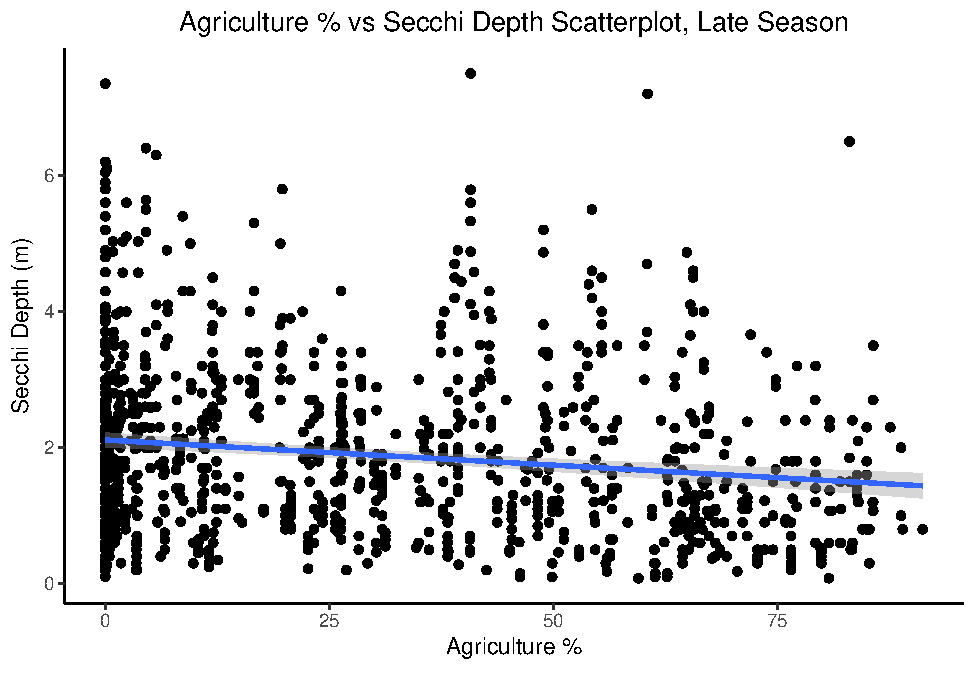
\includegraphics{Final_Wrangling_Doc_files/figure-latex/scatterplots-3.pdf}

\begin{Shaded}
\begin{Highlighting}[]
\KeywordTok{ggplot}\NormalTok{(LAGOS.MN.processed.Late.sf, }\KeywordTok{aes}\NormalTok{(}\DataTypeTok{x =}\NormalTok{ Undeveloped.pct, }\DataTypeTok{y =}\NormalTok{ chla)) }\OperatorTok{+}
\KeywordTok{geom_point}\NormalTok{() }\OperatorTok{+}
\KeywordTok{geom_smooth}\NormalTok{(}\DataTypeTok{method=}\NormalTok{lm) }\OperatorTok{+}
\KeywordTok{xlab}\NormalTok{(}\KeywordTok{expression}\NormalTok{(}\StringTok{"Undeveloped %"}\NormalTok{)) }\OperatorTok{+}
\KeywordTok{ylab}\NormalTok{(}\KeywordTok{expression}\NormalTok{(}\StringTok{"Chla (mg/L)"}\NormalTok{)) }\OperatorTok{+}
\KeywordTok{ggtitle}\NormalTok{(}\StringTok{"Undeveloped % vs Chla Scatterplot, Late Season"}\NormalTok{) }\OperatorTok{+}
\KeywordTok{theme}\NormalTok{(}\DataTypeTok{plot.title =} \KeywordTok{element_text}\NormalTok{(}\DataTypeTok{hjust =} \FloatTok{0.5}\NormalTok{))}
\end{Highlighting}
\end{Shaded}

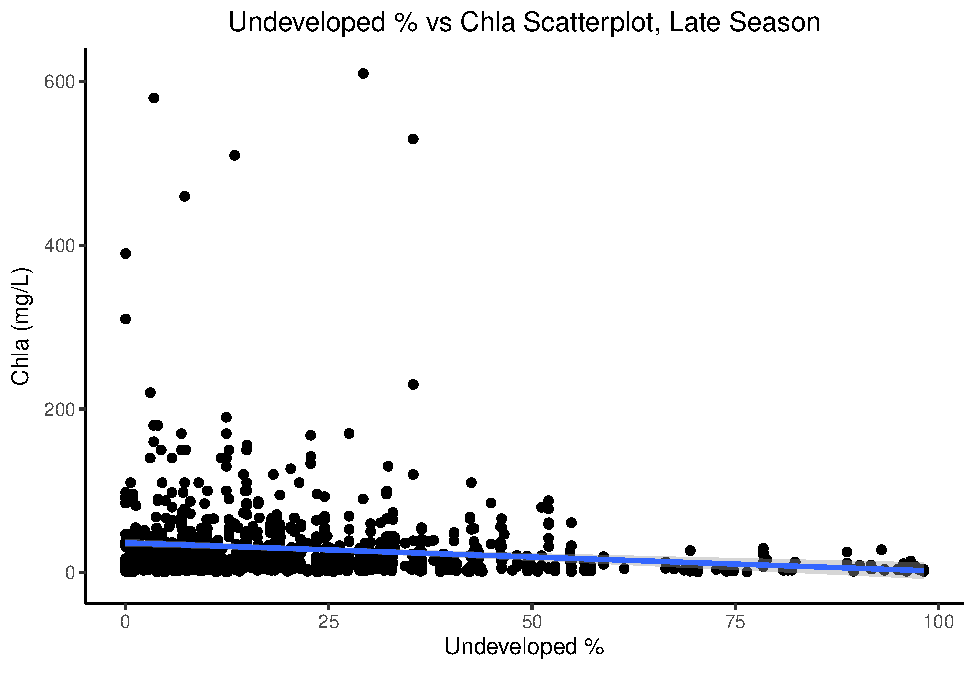
\includegraphics{Final_Wrangling_Doc_files/figure-latex/scatterplots-4.pdf}

\begin{Shaded}
\begin{Highlighting}[]
\KeywordTok{ggplot}\NormalTok{(LAGOS.MN.processed.Late.sf, }\KeywordTok{aes}\NormalTok{(}\DataTypeTok{x =}\NormalTok{ Urban.pct, }\DataTypeTok{y =}\NormalTok{ chla)) }\OperatorTok{+}
\KeywordTok{geom_point}\NormalTok{() }\OperatorTok{+}
\KeywordTok{geom_smooth}\NormalTok{(}\DataTypeTok{method=}\NormalTok{lm) }\OperatorTok{+}
\KeywordTok{xlab}\NormalTok{(}\KeywordTok{expression}\NormalTok{(}\StringTok{"Urban %"}\NormalTok{)) }\OperatorTok{+}
\KeywordTok{ylab}\NormalTok{(}\KeywordTok{expression}\NormalTok{(}\StringTok{"Chla (mg/L)"}\NormalTok{)) }\OperatorTok{+}
\KeywordTok{ggtitle}\NormalTok{(}\StringTok{"Urban % vs Chla Scatterplot, Late Season"}\NormalTok{) }\OperatorTok{+}
\KeywordTok{theme}\NormalTok{(}\DataTypeTok{plot.title =} \KeywordTok{element_text}\NormalTok{(}\DataTypeTok{hjust =} \FloatTok{0.5}\NormalTok{))}
\end{Highlighting}
\end{Shaded}

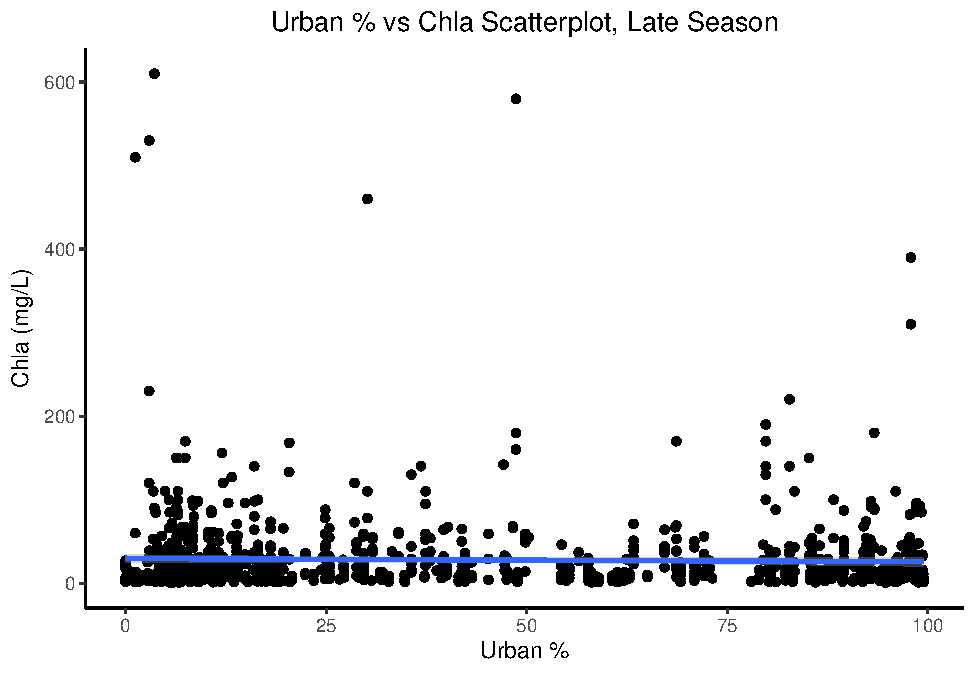
\includegraphics{Final_Wrangling_Doc_files/figure-latex/scatterplots-5.pdf}

\begin{Shaded}
\begin{Highlighting}[]
\KeywordTok{ggplot}\NormalTok{(LAGOS.MN.processed.Late.sf, }\KeywordTok{aes}\NormalTok{(}\DataTypeTok{x =}\NormalTok{ Ag.pct, }\DataTypeTok{y =}\NormalTok{ chla)) }\OperatorTok{+}
\KeywordTok{geom_point}\NormalTok{() }\OperatorTok{+}
\KeywordTok{geom_smooth}\NormalTok{(}\DataTypeTok{method=}\NormalTok{lm) }\OperatorTok{+}
\KeywordTok{xlab}\NormalTok{(}\KeywordTok{expression}\NormalTok{(}\StringTok{"Agriculture %"}\NormalTok{)) }\OperatorTok{+}
\KeywordTok{ylab}\NormalTok{(}\KeywordTok{expression}\NormalTok{(}\StringTok{"Chla (mg/L)"}\NormalTok{)) }\OperatorTok{+}
\KeywordTok{ggtitle}\NormalTok{(}\StringTok{"Agriculture % vs Chla Scatterplot, Late Season"}\NormalTok{) }\OperatorTok{+}
\KeywordTok{theme}\NormalTok{(}\DataTypeTok{plot.title =} \KeywordTok{element_text}\NormalTok{(}\DataTypeTok{hjust =} \FloatTok{0.5}\NormalTok{))}
\end{Highlighting}
\end{Shaded}

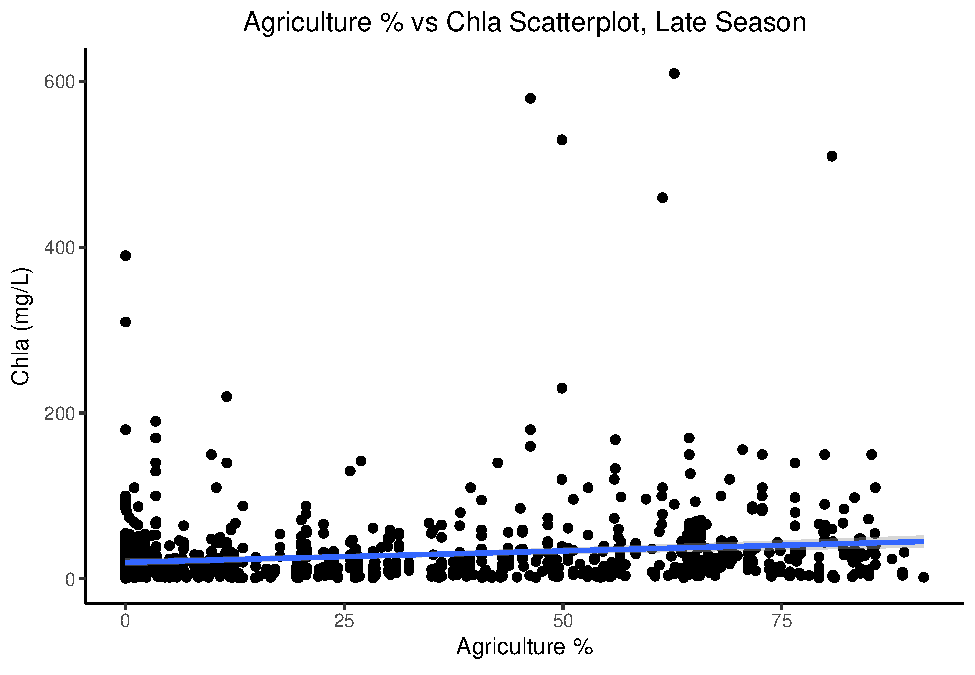
\includegraphics{Final_Wrangling_Doc_files/figure-latex/scatterplots-6.pdf}

\begin{Shaded}
\begin{Highlighting}[]
\NormalTok{LAGOS.MN.Summary.Late <-}\StringTok{ }\NormalTok{LAGOS.MN.processed.Late }\OperatorTok
\KeywordTok{group_by}\NormalTok{(lagoslakeid) }\OperatorTok
\KeywordTok{summarise}\NormalTok{(}\DataTypeTok{secchi.mean =} \KeywordTok{mean}\NormalTok{(secchi),}
          \DataTypeTok{chla.mean =} \KeywordTok{mean}\NormalTok{(chla),}
          \DataTypeTok{lake.area =} \KeywordTok{mean}\NormalTok{(lake_area_ha),}
          \DataTypeTok{iws.area =} \KeywordTok{mean}\NormalTok{(iws_ha),}
          \DataTypeTok{LakeIWS.Ratio =} \KeywordTok{mean}\NormalTok{(LakeIWS.Ratio),}
          \DataTypeTok{Water.pct =} \KeywordTok{mean}\NormalTok{(Water.pct),}
          \DataTypeTok{Urban.pct =} \KeywordTok{mean}\NormalTok{(Urban.pct),}
          \DataTypeTok{Undeveloped.pct =} \KeywordTok{mean}\NormalTok{(Undeveloped.pct),}
          \DataTypeTok{Ag.pct =} \KeywordTok{mean}\NormalTok{(Ag.pct),}
          \DataTypeTok{Lat =} \KeywordTok{mean}\NormalTok{(nhd_lat),}
          \DataTypeTok{Long =} \KeywordTok{mean}\NormalTok{(nhd_long)}
\NormalTok{          ) }\OperatorTok
\StringTok{  }\KeywordTok{drop_na}\NormalTok{()}

\CommentTok{#SF file with the summary}
\NormalTok{LAGOS.MN.Summary.Late.sf <-}\StringTok{ }\KeywordTok{st_as_sf}\NormalTok{(LAGOS.MN.Summary.Late, }\DataTypeTok{coords =} \KeywordTok{c}\NormalTok{(}\StringTok{"Long"}\NormalTok{, }\StringTok{"Lat"}\NormalTok{), }\DataTypeTok{crs =} \DecValTok{4326}\NormalTok{)}


\CommentTok{#Loading the MN state boundary  }
\CommentTok{# generate a map of U.S. states}
\NormalTok{states <-}\StringTok{ }\KeywordTok{st_as_sf}\NormalTok{(}\KeywordTok{map}\NormalTok{(}\DataTypeTok{database =} \StringTok{"state"}\NormalTok{, }\DataTypeTok{plot =} \OtherTok{FALSE}\NormalTok{, }\DataTypeTok{fill =} \OtherTok{TRUE}\NormalTok{, }\DataTypeTok{col =} \StringTok{"white"}\NormalTok{))}

\CommentTok{# filter MN}
\NormalTok{states.MN <-}\StringTok{ }\KeywordTok{filter}\NormalTok{(states, ID }\OperatorTok
\KeywordTok{c}\NormalTok{(}\StringTok{"minnesota"}\NormalTok{))}

\NormalTok{secchiplot1.Late.MN <-}\StringTok{ }\KeywordTok{ggplot}\NormalTok{() }\OperatorTok{+}
\StringTok{  }\KeywordTok{geom_sf}\NormalTok{(}\DataTypeTok{data =}\NormalTok{ states.MN, }\DataTypeTok{fill =} \StringTok{"white"}\NormalTok{) }\OperatorTok{+}
\StringTok{  }\KeywordTok{geom_sf}\NormalTok{(}\DataTypeTok{data =}\NormalTok{ LAGOS.MN.Summary.Late.sf, }
          \KeywordTok{aes}\NormalTok{(}\DataTypeTok{size =}\NormalTok{ Undeveloped.pct, }\DataTypeTok{color =}\NormalTok{ secchi.mean),}
          \DataTypeTok{alpha =} \FloatTok{0.4}\NormalTok{, }\DataTypeTok{show.legend =} \StringTok{"point"}\NormalTok{) }\OperatorTok{+}
\StringTok{  }\KeywordTok{scale_color_viridis_c}\NormalTok{(}\DataTypeTok{option =} \StringTok{"inferno"}\NormalTok{) }\OperatorTok{+}
\StringTok{  }\KeywordTok{labs}\NormalTok{(}\DataTypeTok{color =} \StringTok{"Average }\CharTok{\textbackslash{}n}\StringTok{ Secchi }\CharTok{\textbackslash{}n}\StringTok{ Depth (m)"}\NormalTok{, }
       \DataTypeTok{size =} \StringTok{"Undeveloped }\CharTok{\textbackslash{}n}\StringTok{ Area }\CharTok{\textbackslash{}n}\StringTok{ %"}\NormalTok{) }\OperatorTok{+}
\StringTok{  }\KeywordTok{theme}\NormalTok{(}\DataTypeTok{legend.position =} \StringTok{"right"}\NormalTok{, }\DataTypeTok{legend.text =} \KeywordTok{element_text}\NormalTok{(}\DataTypeTok{size =} \DecValTok{7}\NormalTok{),}
        \DataTypeTok{legend.title =} \KeywordTok{element_text}\NormalTok{(}\DataTypeTok{size =} \DecValTok{8}\NormalTok{),}
        \DataTypeTok{legend.margin =} \KeywordTok{margin}\NormalTok{(}\DecValTok{0}\NormalTok{,}\DecValTok{0}\NormalTok{,}\DecValTok{0}\NormalTok{,}\DecValTok{0}\NormalTok{)) }
\KeywordTok{print}\NormalTok{(secchiplot1.Late.MN)}
\end{Highlighting}
\end{Shaded}

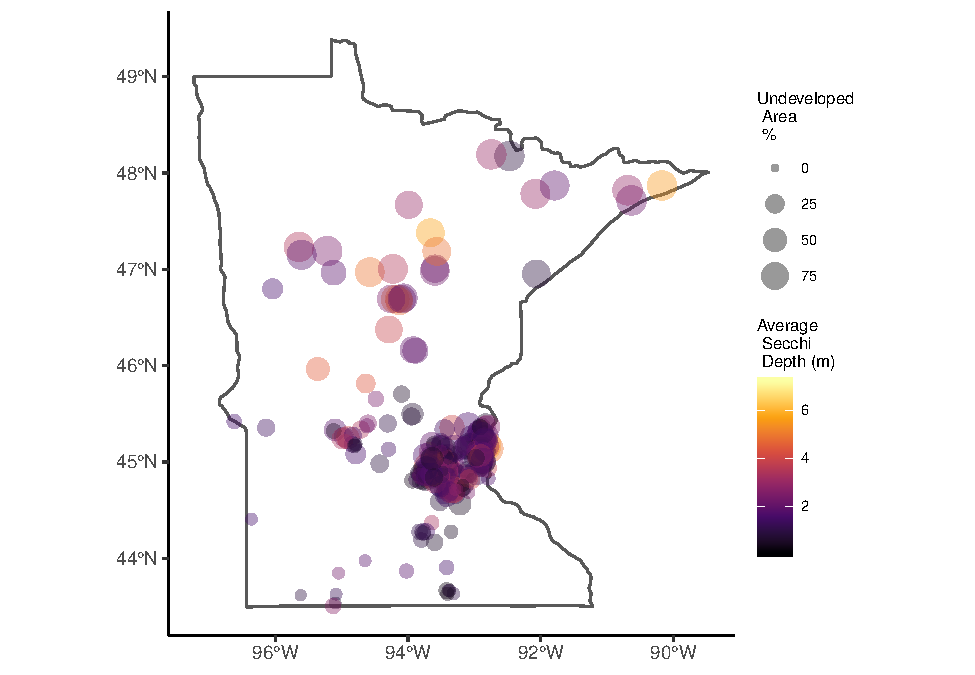
\includegraphics{Final_Wrangling_Doc_files/figure-latex/summary.for.late.season-1.pdf}

\begin{Shaded}
\begin{Highlighting}[]
\NormalTok{secchiplot2.Late.MN <-}\StringTok{ }\KeywordTok{ggplot}\NormalTok{() }\OperatorTok{+}
\StringTok{  }\KeywordTok{geom_sf}\NormalTok{(}\DataTypeTok{data =}\NormalTok{ states.MN, }\DataTypeTok{fill =} \StringTok{"white"}\NormalTok{) }\OperatorTok{+}
\StringTok{  }\KeywordTok{geom_sf}\NormalTok{(}\DataTypeTok{data =}\NormalTok{ LAGOS.MN.Summary.Late.sf, }
          \KeywordTok{aes}\NormalTok{(}\DataTypeTok{size =}\NormalTok{ Urban.pct, }\DataTypeTok{color =}\NormalTok{ secchi.mean),}
          \DataTypeTok{alpha =} \FloatTok{0.4}\NormalTok{, }\DataTypeTok{show.legend =} \StringTok{"point"}\NormalTok{) }\OperatorTok{+}
\StringTok{  }\KeywordTok{scale_color_viridis_c}\NormalTok{(}\DataTypeTok{option =} \StringTok{"inferno"}\NormalTok{) }\OperatorTok{+}
\StringTok{  }\KeywordTok{labs}\NormalTok{(}\DataTypeTok{color =} \StringTok{"Average }\CharTok{\textbackslash{}n}\StringTok{ Secchi }\CharTok{\textbackslash{}n}\StringTok{ Depth (m)"}\NormalTok{, }
       \DataTypeTok{size =} \StringTok{"Urban }\CharTok{\textbackslash{}n}\StringTok{ Area }\CharTok{\textbackslash{}n}\StringTok{ %"}\NormalTok{) }\OperatorTok{+}
\StringTok{  }\KeywordTok{theme}\NormalTok{(}\DataTypeTok{legend.position =} \StringTok{"right"}\NormalTok{, }\DataTypeTok{legend.text =} \KeywordTok{element_text}\NormalTok{(}\DataTypeTok{size =} \DecValTok{7}\NormalTok{),}
        \DataTypeTok{legend.title =} \KeywordTok{element_text}\NormalTok{(}\DataTypeTok{size =} \DecValTok{8}\NormalTok{),}
        \DataTypeTok{legend.margin =} \KeywordTok{margin}\NormalTok{(}\DecValTok{0}\NormalTok{,}\DecValTok{0}\NormalTok{,}\DecValTok{0}\NormalTok{,}\DecValTok{0}\NormalTok{)) }
\KeywordTok{print}\NormalTok{(secchiplot2.Late.MN)}
\end{Highlighting}
\end{Shaded}

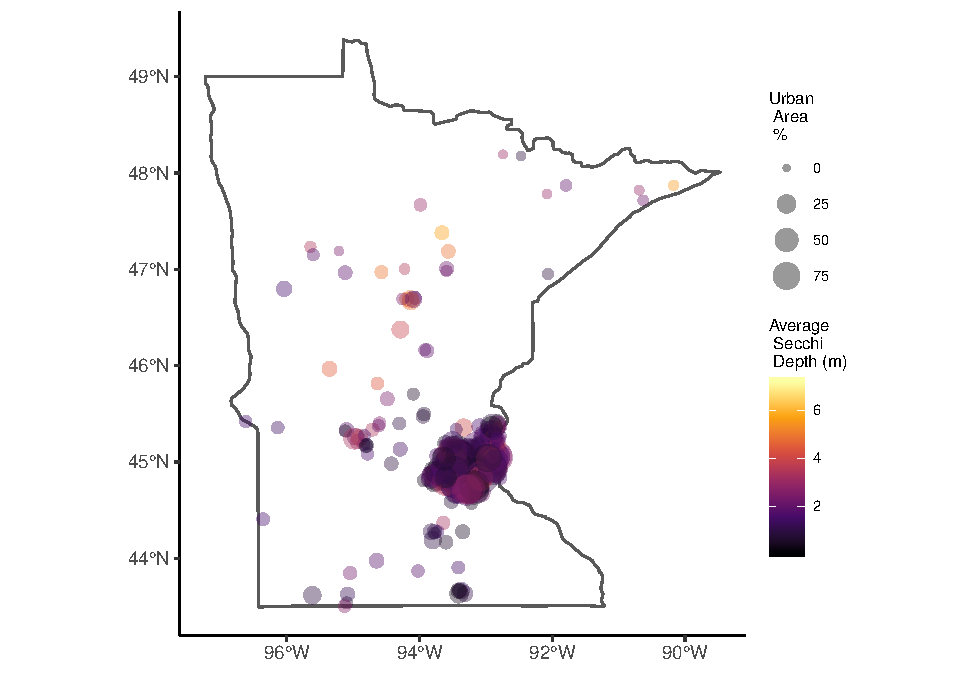
\includegraphics{Final_Wrangling_Doc_files/figure-latex/summary.for.late.season-2.pdf}

\begin{Shaded}
\begin{Highlighting}[]
\NormalTok{secchiplot3.Late.MN <-}\StringTok{ }\KeywordTok{ggplot}\NormalTok{() }\OperatorTok{+}
\StringTok{  }\KeywordTok{geom_sf}\NormalTok{(}\DataTypeTok{data =}\NormalTok{ states.MN, }\DataTypeTok{fill =} \StringTok{"white"}\NormalTok{) }\OperatorTok{+}
\StringTok{  }\KeywordTok{geom_sf}\NormalTok{(}\DataTypeTok{data =}\NormalTok{ LAGOS.MN.Summary.Late.sf, }
          \KeywordTok{aes}\NormalTok{(}\DataTypeTok{size =}\NormalTok{ Ag.pct, }\DataTypeTok{color =}\NormalTok{ secchi.mean),}
          \DataTypeTok{alpha =} \FloatTok{0.4}\NormalTok{, }\DataTypeTok{show.legend =} \StringTok{"point"}\NormalTok{) }\OperatorTok{+}
\StringTok{  }\KeywordTok{scale_color_viridis_c}\NormalTok{(}\DataTypeTok{option =} \StringTok{"inferno"}\NormalTok{) }\OperatorTok{+}
\StringTok{  }\KeywordTok{labs}\NormalTok{(}\DataTypeTok{color =} \StringTok{"Average }\CharTok{\textbackslash{}n}\StringTok{ Secchi }\CharTok{\textbackslash{}n}\StringTok{ Depth (m)"}\NormalTok{, }
       \DataTypeTok{size =} \StringTok{"Agricultural }\CharTok{\textbackslash{}n}\StringTok{ Area }\CharTok{\textbackslash{}n}\StringTok{ %"}\NormalTok{) }\OperatorTok{+}
\StringTok{  }\KeywordTok{theme}\NormalTok{(}\DataTypeTok{legend.position =} \StringTok{"right"}\NormalTok{, }\DataTypeTok{legend.text =} \KeywordTok{element_text}\NormalTok{(}\DataTypeTok{size =} \DecValTok{7}\NormalTok{),}
        \DataTypeTok{legend.title =} \KeywordTok{element_text}\NormalTok{(}\DataTypeTok{size =} \DecValTok{8}\NormalTok{),}
        \DataTypeTok{legend.margin =} \KeywordTok{margin}\NormalTok{(}\DecValTok{0}\NormalTok{,}\DecValTok{0}\NormalTok{,}\DecValTok{0}\NormalTok{,}\DecValTok{0}\NormalTok{)) }
\KeywordTok{print}\NormalTok{(secchiplot3.Late.MN)}
\end{Highlighting}
\end{Shaded}

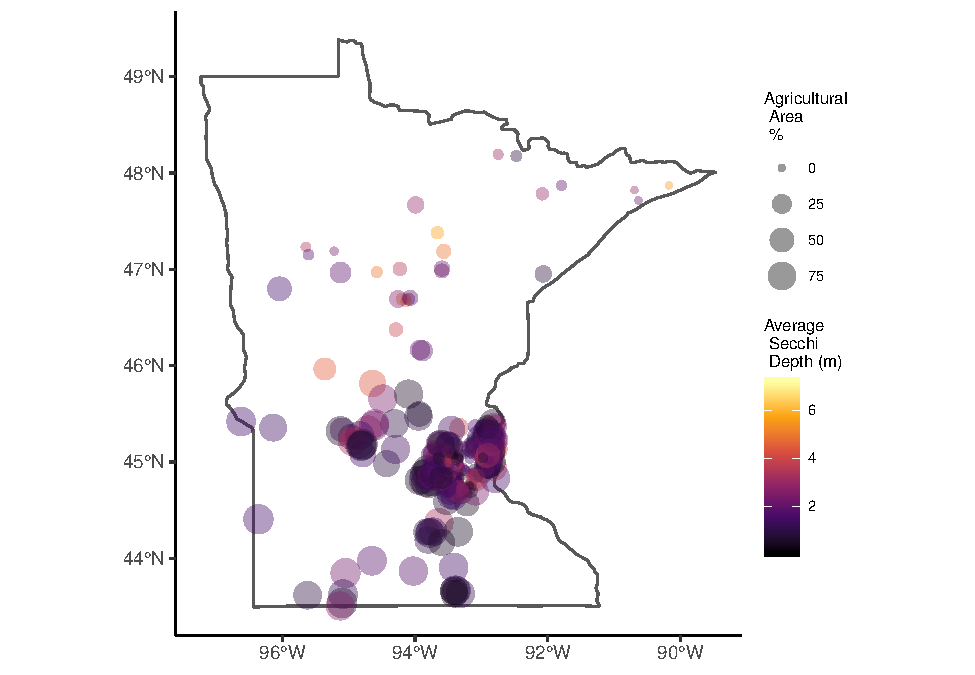
\includegraphics{Final_Wrangling_Doc_files/figure-latex/summary.for.late.season-3.pdf}

\begin{Shaded}
\begin{Highlighting}[]
\NormalTok{chlaplot1.Late.MN <-}\StringTok{ }\KeywordTok{ggplot}\NormalTok{() }\OperatorTok{+}
\StringTok{  }\KeywordTok{geom_sf}\NormalTok{(}\DataTypeTok{data =}\NormalTok{ states.MN, }\DataTypeTok{fill =} \StringTok{"white"}\NormalTok{) }\OperatorTok{+}
\StringTok{  }\KeywordTok{geom_sf}\NormalTok{(}\DataTypeTok{data =}\NormalTok{ LAGOS.MN.Summary.Late.sf, }
          \KeywordTok{aes}\NormalTok{(}\DataTypeTok{size =}\NormalTok{ Undeveloped.pct, }\DataTypeTok{color =}\NormalTok{ chla.mean),}
          \DataTypeTok{alpha =} \FloatTok{0.4}\NormalTok{, }\DataTypeTok{show.legend =} \StringTok{"point"}\NormalTok{) }\OperatorTok{+}
\StringTok{  }\KeywordTok{scale_color_viridis_c}\NormalTok{(}\DataTypeTok{option =} \StringTok{"inferno"}\NormalTok{) }\OperatorTok{+}
\StringTok{  }\KeywordTok{labs}\NormalTok{(}\DataTypeTok{color =} \StringTok{"Average }\CharTok{\textbackslash{}n}\StringTok{ Chla }\CharTok{\textbackslash{}n}\StringTok{ Depth (m)"}\NormalTok{, }
       \DataTypeTok{size =} \StringTok{"Undeveloped }\CharTok{\textbackslash{}n}\StringTok{ Area }\CharTok{\textbackslash{}n}\StringTok{ %"}\NormalTok{) }\OperatorTok{+}
\StringTok{  }\KeywordTok{theme}\NormalTok{(}\DataTypeTok{legend.position =} \StringTok{"right"}\NormalTok{, }\DataTypeTok{legend.text =} \KeywordTok{element_text}\NormalTok{(}\DataTypeTok{size =} \DecValTok{7}\NormalTok{),}
        \DataTypeTok{legend.title =} \KeywordTok{element_text}\NormalTok{(}\DataTypeTok{size =} \DecValTok{8}\NormalTok{),}
        \DataTypeTok{legend.margin =} \KeywordTok{margin}\NormalTok{(}\DecValTok{0}\NormalTok{,}\DecValTok{0}\NormalTok{,}\DecValTok{0}\NormalTok{,}\DecValTok{0}\NormalTok{)) }
\KeywordTok{print}\NormalTok{(chlaplot1.Late.MN)}
\end{Highlighting}
\end{Shaded}

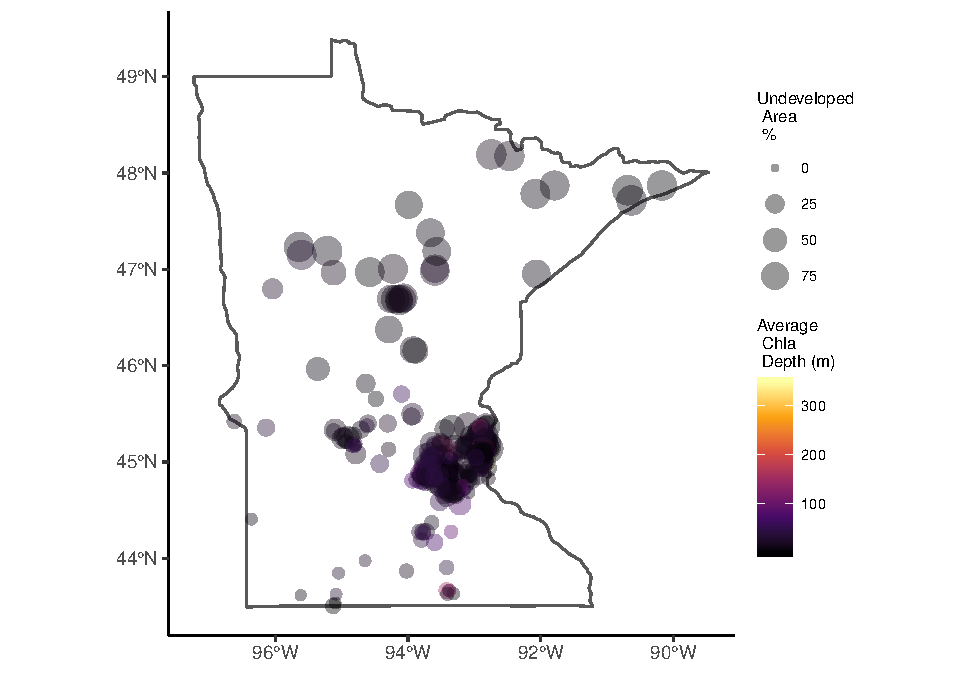
\includegraphics{Final_Wrangling_Doc_files/figure-latex/summary.for.late.season-4.pdf}

\begin{Shaded}
\begin{Highlighting}[]
\NormalTok{chlaplot2.Late.MN <-}\StringTok{ }\KeywordTok{ggplot}\NormalTok{() }\OperatorTok{+}
\StringTok{  }\KeywordTok{geom_sf}\NormalTok{(}\DataTypeTok{data =}\NormalTok{ states.MN, }\DataTypeTok{fill =} \StringTok{"white"}\NormalTok{) }\OperatorTok{+}
\StringTok{  }\KeywordTok{geom_sf}\NormalTok{(}\DataTypeTok{data =}\NormalTok{ LAGOS.MN.Summary.Late.sf, }
          \KeywordTok{aes}\NormalTok{(}\DataTypeTok{size =}\NormalTok{ Urban.pct, }\DataTypeTok{color =}\NormalTok{ chla.mean),}
          \DataTypeTok{alpha =} \FloatTok{0.4}\NormalTok{, }\DataTypeTok{show.legend =} \StringTok{"point"}\NormalTok{) }\OperatorTok{+}
\StringTok{  }\KeywordTok{scale_color_viridis_c}\NormalTok{(}\DataTypeTok{option =} \StringTok{"inferno"}\NormalTok{) }\OperatorTok{+}
\StringTok{  }\KeywordTok{labs}\NormalTok{(}\DataTypeTok{color =} \StringTok{"Average }\CharTok{\textbackslash{}n}\StringTok{ Chla }\CharTok{\textbackslash{}n}\StringTok{ Depth (m)"}\NormalTok{, }
       \DataTypeTok{size =} \StringTok{"Urban }\CharTok{\textbackslash{}n}\StringTok{ Area }\CharTok{\textbackslash{}n}\StringTok{ %"}\NormalTok{) }\OperatorTok{+}
\StringTok{  }\KeywordTok{theme}\NormalTok{(}\DataTypeTok{legend.position =} \StringTok{"right"}\NormalTok{, }\DataTypeTok{legend.text =} \KeywordTok{element_text}\NormalTok{(}\DataTypeTok{size =} \DecValTok{7}\NormalTok{),}
        \DataTypeTok{legend.title =} \KeywordTok{element_text}\NormalTok{(}\DataTypeTok{size =} \DecValTok{8}\NormalTok{),}
        \DataTypeTok{legend.margin =} \KeywordTok{margin}\NormalTok{(}\DecValTok{0}\NormalTok{,}\DecValTok{0}\NormalTok{,}\DecValTok{0}\NormalTok{,}\DecValTok{0}\NormalTok{)) }
\KeywordTok{print}\NormalTok{(chlaplot2.Late.MN)}
\end{Highlighting}
\end{Shaded}

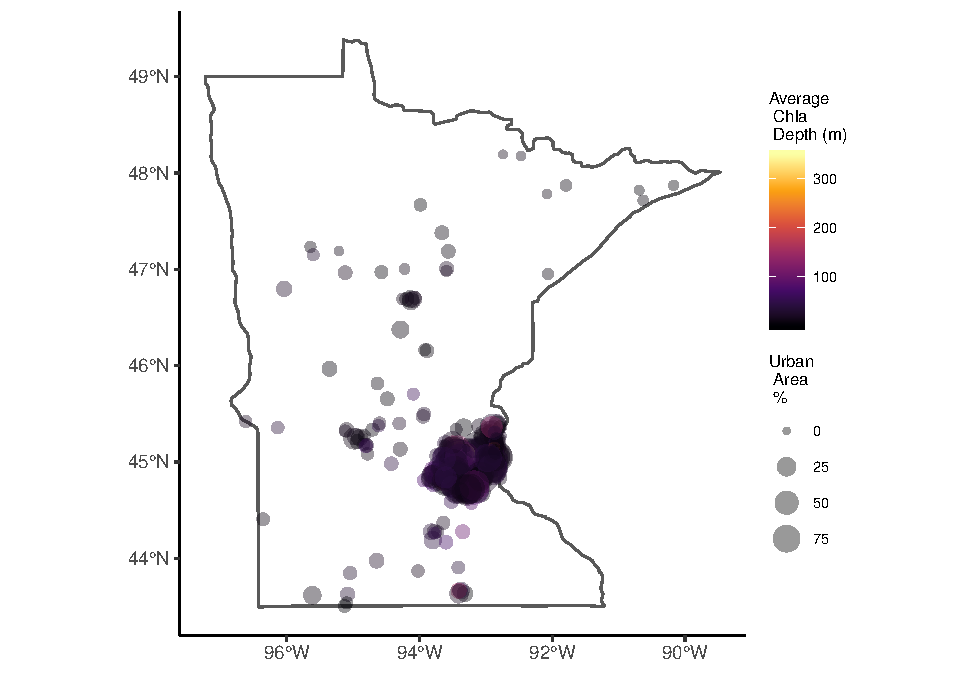
\includegraphics{Final_Wrangling_Doc_files/figure-latex/summary.for.late.season-5.pdf}

\begin{Shaded}
\begin{Highlighting}[]
\NormalTok{chlaplot3.Late.MN <-}\StringTok{ }\KeywordTok{ggplot}\NormalTok{() }\OperatorTok{+}
\StringTok{  }\KeywordTok{geom_sf}\NormalTok{(}\DataTypeTok{data =}\NormalTok{ states.MN, }\DataTypeTok{fill =} \StringTok{"white"}\NormalTok{) }\OperatorTok{+}
\StringTok{  }\KeywordTok{geom_sf}\NormalTok{(}\DataTypeTok{data =}\NormalTok{ LAGOS.MN.Summary.Late.sf, }
          \KeywordTok{aes}\NormalTok{(}\DataTypeTok{size =}\NormalTok{ Ag.pct, }\DataTypeTok{color =}\NormalTok{ chla.mean),}
          \DataTypeTok{alpha =} \FloatTok{0.4}\NormalTok{, }\DataTypeTok{show.legend =} \StringTok{"point"}\NormalTok{) }\OperatorTok{+}
\StringTok{  }\KeywordTok{scale_color_viridis_c}\NormalTok{(}\DataTypeTok{option =} \StringTok{"inferno"}\NormalTok{) }\OperatorTok{+}
\StringTok{  }\KeywordTok{labs}\NormalTok{(}\DataTypeTok{color =} \StringTok{"Average }\CharTok{\textbackslash{}n}\StringTok{ Chla }\CharTok{\textbackslash{}n}\StringTok{ Depth (m)"}\NormalTok{, }
       \DataTypeTok{size =} \StringTok{"Agricultural }\CharTok{\textbackslash{}n}\StringTok{ Area }\CharTok{\textbackslash{}n}\StringTok{ %"}\NormalTok{) }\OperatorTok{+}
\StringTok{  }\KeywordTok{theme}\NormalTok{(}\DataTypeTok{legend.position =} \StringTok{"right"}\NormalTok{, }\DataTypeTok{legend.text =} \KeywordTok{element_text}\NormalTok{(}\DataTypeTok{size =} \DecValTok{7}\NormalTok{),}
        \DataTypeTok{legend.title =} \KeywordTok{element_text}\NormalTok{(}\DataTypeTok{size =} \DecValTok{8}\NormalTok{),}
        \DataTypeTok{legend.margin =} \KeywordTok{margin}\NormalTok{(}\DecValTok{0}\NormalTok{,}\DecValTok{0}\NormalTok{,}\DecValTok{0}\NormalTok{,}\DecValTok{0}\NormalTok{)) }
\KeywordTok{print}\NormalTok{(secchiplot3.Late.MN)}
\end{Highlighting}
\end{Shaded}

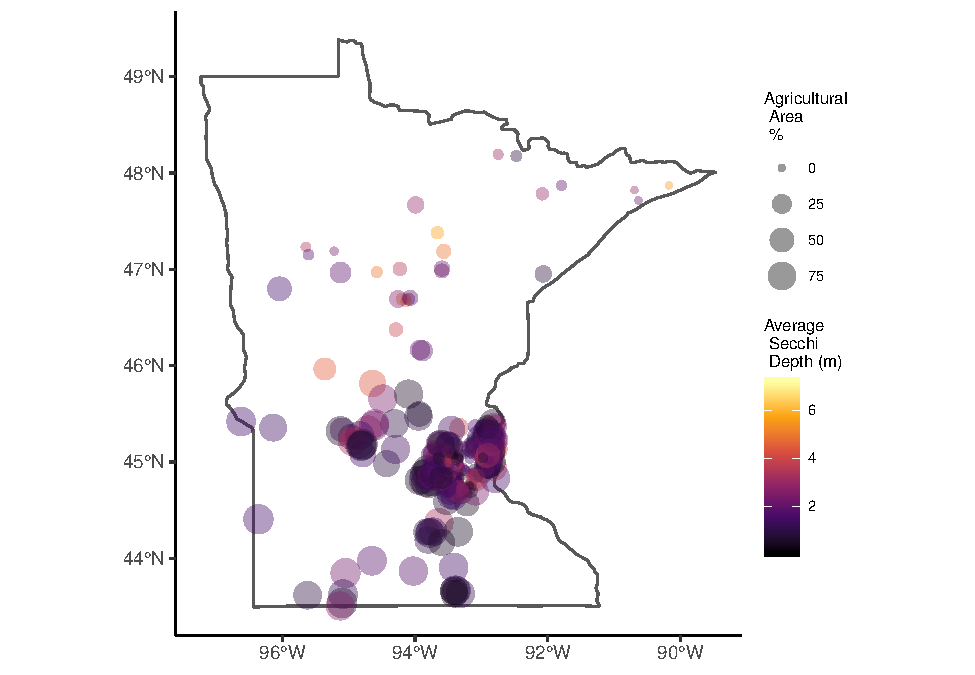
\includegraphics{Final_Wrangling_Doc_files/figure-latex/summary.for.late.season-6.pdf}

\begin{Shaded}
\begin{Highlighting}[]
\KeywordTok{st_geometry}\NormalTok{(LAGOS.MN.processed.Early.sf) <-}\StringTok{ }\OtherTok{NULL}
\KeywordTok{write.csv}\NormalTok{(}\DataTypeTok{x =}\NormalTok{  LAGOS.MN.processed.Early.sf, }\DataTypeTok{row.names =} \OtherTok{FALSE}\NormalTok{,}
          \DataTypeTok{file =}  \StringTok{"./data/processed/LAGOS.MN.processed.Early.csv"}\NormalTok{)}

\KeywordTok{st_geometry}\NormalTok{(LAGOS.MN.processed.Prime.sf) <-}\StringTok{ }\OtherTok{NULL}
\KeywordTok{write.csv}\NormalTok{(}\DataTypeTok{x =}\NormalTok{  LAGOS.MN.processed.Prime.sf, }\DataTypeTok{row.names =} \OtherTok{FALSE}\NormalTok{,}
          \DataTypeTok{file =}  \StringTok{"./data/processed/LAGOS.MN.processed.Prime.csv"}\NormalTok{)}

\KeywordTok{st_geometry}\NormalTok{(LAGOS.MN.processed.Late.sf) <-}\StringTok{ }\OtherTok{NULL}
\KeywordTok{write.csv}\NormalTok{(}\DataTypeTok{x =}\NormalTok{  LAGOS.MN.processed.Late.sf, }\DataTypeTok{row.names =} \OtherTok{FALSE}\NormalTok{,}
          \DataTypeTok{file =}  \StringTok{"./data/processed/LAGOS.MN.processed.Late.csv"}\NormalTok{)}
\end{Highlighting}
\end{Shaded}


\end{document}
